\section{Evaluation}
\subsection{Offline Classification Performance}
%\todo[inline]{RD: TODO for @LK: Provide the results that were collected when testing offline}
%The SVM model training software is implemented to enable the use of a variable constellation of logged datasets. Moreover, it can be used to compare both the offline and online classification performance.
The components of a Linear Discriminant Analysis (\emph{LDA}) are plotted to visualize the achieved data separation. 
In the LDA two Linear Discriminant components are represented on the axes. These components are formed from a reduction of the original feature set.
Figure~\ref{fig:LDA} shows a LDA plot of the dataset and highlights the decision boundary of the trained linear SVM kernel. 
The areas of different terrain types are highlighted by the corresponding colors. 
It is shown that the data of the terrain types can be separated for most of the samples.

The offline evaluation of the SVM classifier reaches an accuracy of 93.97\%, depicted in the confusion matrix in Figure~\ref{fig:CM}. 
A small portion of the collected data where SherpaTT was not moving was manually removed. 
Based on the sliced data the classification accuracy is increased by 2\%.
Except the recall for \emph{compact sand} and the precision for \emph{sand} all performances are above 90\%, with an overall accuracy of 93.97\%.


\begin{figure}
    \centering
    {\includegraphics[width=\columnwidth]{../figures/boundary_LDA_prevTesting_all_sand_concrete_compactsand.png}}
    \caption{Linear Discriminant Analysis of the dataset. The decision boundaries of linear SVC for three examined terrain types are highlighted with colors: concrete (blue), compact sand (grey) and loose sand (red).}
    \label{fig:LDA}
\end{figure}

\begin{figure}
    \centering
    {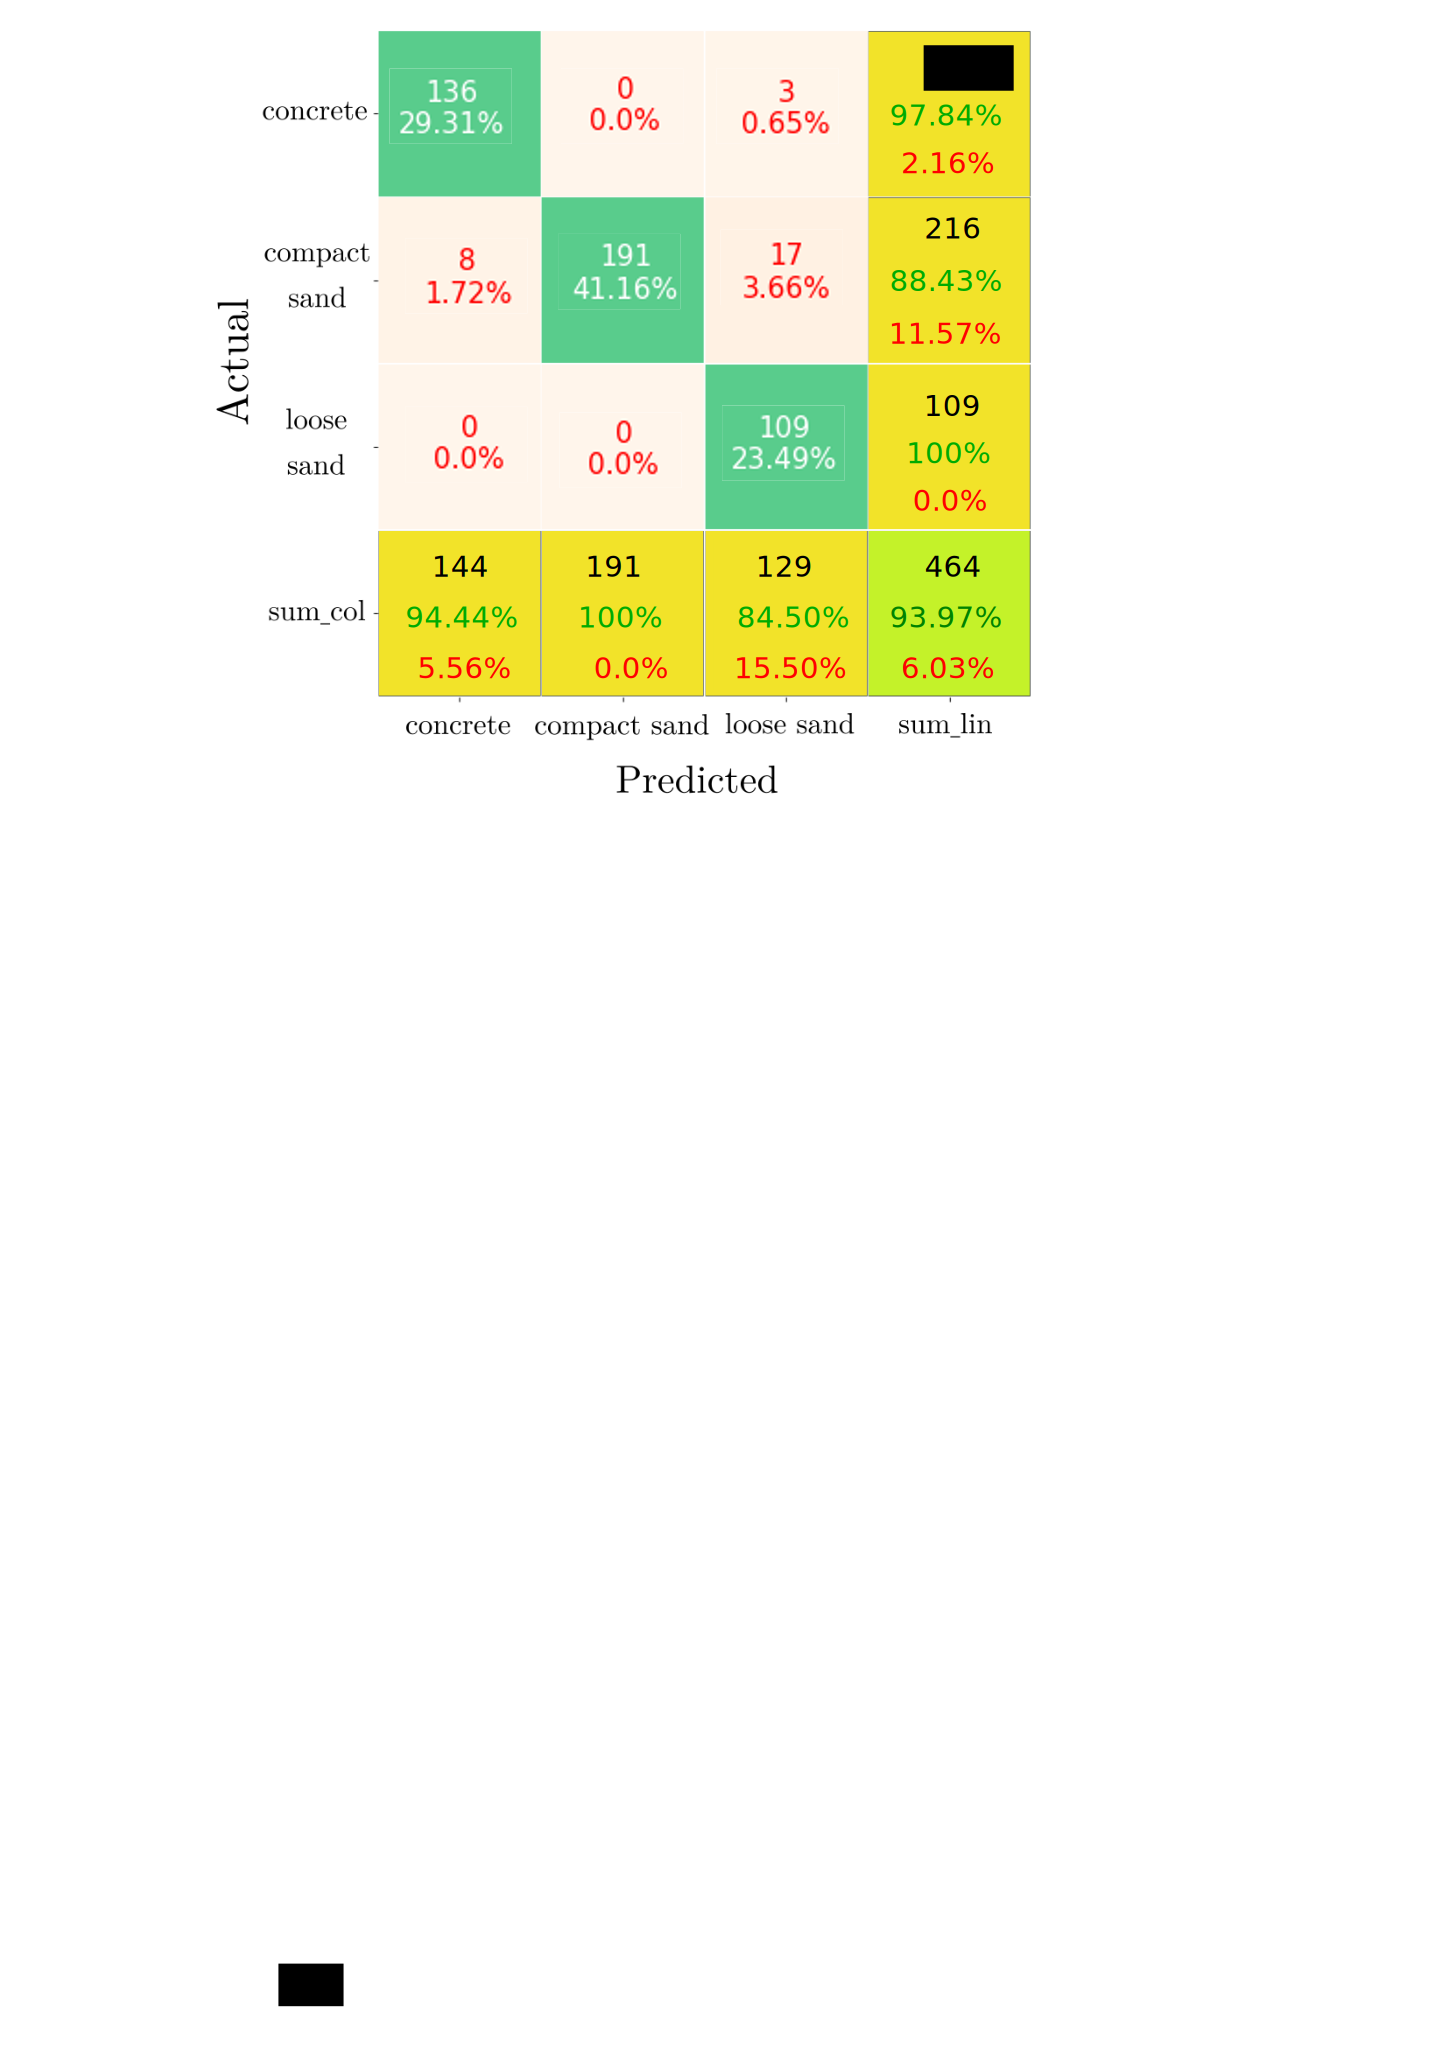
\includegraphics[width=\columnwidth]{../figures/confusionmatrix_Train_yellow.png}}
    \caption{ The confusion matrix of the terrain classifier shows the performance of the SVM model with respect to the different terrain types. The overall accuracy yields 93.97\% }
    \label{fig:CM}
\end{figure}


%\FloatBarrier
% Evaluation

%A complete analysis of performance was not possible, because the traversed terrain during the field tests did not closly match the previously trained terrain classes. Nevertheless, the software shows good classification results, since the type of surface -\emph{wet compact sand}- was close to the two classes mostly identified -\emph{concrete} and \emph{compact sand}.

\subsection{On-Board tests}

Two main tests were performed to validate the on-board feature calculation and classification performance. The software components were running in parallel with the rest of the control and perception software while the rover was traversing
the test area.

The first test was excecuteed indoors at the DFKI Robotics Innovation Center premises, depicted in Figure~\ref{fig:sh-tests}.
During the test, the classifier ran at the pursued frequency of 100~$\mathit{Hz}$.
Nevertheless, the classification performance of these tests is not considered representative, since the power generator was not active and the hardest surface was not as firm as concrete. 

\begin{figure}[!htbp]
    \begin{center}
    \subcaptionbox
        {Loose Sand Tests}
        {
            \includegraphics[width=\columnwidth]{../figures/spacehall.png}
        }
    \subcaptionbox
        {Concrete Tests}
        {
            \includegraphics[width=\columnwidth]{../figures/spacehallconcrete.png}
        }
    \end{center}
    \caption{Validation of execution frequencies for the on-board terrain classifier.}
    \label{fig:sh-tests}
\end{figure}

The second test took place during the final field trials of the ADE project \cite{ocon2021} in a sand mine in Wulsbüttel, Northern Germany.
These test runs provided comparable conditions with the ones within the training data set, because the power generator was activated. 
Several traverses of the SherpaTT rover were logged and checked for consistency to validate the feature calculation. 
The classification accuracy reached 87\%. Well balanced recall and precision values of the classes were also achieved. 
The underperformance in the field tests can be explained by the encountered surface conditions, which did not closely match any of the previously examined surface types. 
Due to rainfalls, the surface turned into wet compact soil and sticked to the wheels as shown in Figure~\ref{fig:finaltest}, causing unaccounted dynamics.
Nevertheless, the classification resulted in 87.69\% \emph{concrete} and 12.31\% \emph{compact sand}, complying with the closest types of terrain the classifier was trained with.
The field trials demonstrated that the terrain classifier can be executed on-board of SherpaTT, that it is able to compute correct features and to classify different terrain types successfully while the rover is traversing a surface.

\begin{figure}[!htbp]
    \centering
        \includegraphics[width=\columnwidth]{../figures/sandmine.jpg}
    \caption{The analog site where the classifier was tested.}
    \label{fig:finaltest}
\end{figure}


\subsection{Computational Performance}
The execution time of the code has been repeatedly measured. 
Since the computation is executed on a single thread, the execution time can be identified measuring the averaged wall time of the code execution. 
The resulting execution time depends on the threading of the operating system which in this case is the Linux distribution Ubuntu 18.04 LTS. The time measures were taken on an i7 processor with a CPU clock speed of 4.6 GHz. 
Table~\ref{table:compmeasurments} shows the results of these measurements. 

\begin{center}
\bottomcaption{Wall time measurements of the methods of the C++ classification library.}
\label{table:compmeasurments}
\tablefirsthead{
        \quad                        & \multicolumn{3}{c}{Wall Time [$ms$]} \\
        \textbf{Method:}             & min.   & max.   & avg.\\ \hline \hline
   }
\begin{supertabular}{r|ccc}
        \quad                         & \quad & \quad & \quad  \\[-5pt]
        \textbf{calculateFeatures():} & 9     & 17.1  & 13.2   \\
        \textbf{calculateStat():}     & 6.3   & 13    & 7.1    \\
        \textbf{svmPredict():}        & 0.0   & 0.001 & 0.0007 \\
        \hline
        \quad                         & \quad & \quad & \quad  \\[-5pt]
        \textbf{overall:}             & 15.3 & 30.1 &20.3  \\
\end{supertabular}
\end{center}

As the averaged execution time of the C++ classification library is 20.3 $ms$ this can lead to a delay of the next data collection step which is repeated every 10 $ms$ and hence can cause the drop of one data sample per second. 
The drop of one data sample out of the one hundred data samples that are strapped every second is assessed to be acceptable.
